\chapter{Background}
\label{chap-background}
\begin{ChapAbstract}
In this chapter, we discuss all necessary background knowledge related to our work. First of all, we start with the very beginning concept in machine learning and then introduce some fundamental models used in processing complex data such as time-series or digital images. Then we introduce a list of Computer Vision problems which play an important role in our proposed approach. 
\end{ChapAbstract}


\section{CT Volume Image}
% ref https://www.ncbi.nlm.nih.gov/books/NBK574548/
CT images are two-dimensional pictures that represent three-dimensional physical objects. The images are made by converting electrical energy (moving electrons) into X-ray photons, passing the photons through an object, and then converting the measured photons back into electrons. The number of X-rays that pass through the object is inversely proportional to the density of the object. Objects imaged by CT consist of parts that vary in density. 

Image slices can either be displayed individually or stacked together by the computer to generate a 3D image of the patient that shows the skeleton, organs, and tissues as well as any abnormalities the physician is trying to identify. This method has many advantages make doctors easier to find the exact place where a problem may be located or identification of basic structures as well as possible tumors or abnormalities.

\subsection{Digital image representation}
% - how the computer store the images ?
In machine computing, image is a well-known definition. The image is construct by multiple pixels, each of them contains multiple values representing its visual information. The value range is often between from 0 to 255, for example it can handle the image brightness or the affect of a specific color (in a colored image). 
% insert image rgb 
Every image is define by structure information, such as image shape like channel, width, height. If the number of channel is 1, the image should be grayscale. And in color image, the number of channel would be 3 (corresponding with red, green and blue). And there are multiple variants of image type, like medical image shape would be constructed by width, height and depth. The depth channel could be thousand and pixel value range could be a negative number.
% insert volume image
\subsection{Hounsfield Units}
The CT detectors measure the degree that the scanned tissues physical density, and the image processor storing the data as pixels calculated by to convert byte data into a range of 5000 values. The scale's range of values is named for Hounsfield; each value on the scale is termed a Hounsfield unit (HU). Densities of various substances have been assigned relative values. The density of the substances in the patient (both natural tissues and any medical implants) and around the patient are calculated based on a linear transformation of the measured \textbf{X-ray attenuation coefficients}. This transformation is based on the standard density measurement of two substances, distilled water (set as 0 HU) and air (set as -1000 HU). HU for various scanned tissues are computed from the following equation: 
\begin{equation}
    HU = 1000 \times (tissue \mu - water \mu)/ water \mu 
\end{equation}
Where $\mu$ is the linear attenuation coefficient. CT scanners used in medical practice can present HU within a range of –1024 HU to +3071 HU. Different publications define different ranges for certain tissues and substances.

% Tissue physical density is proportional to photon attenuation (photon absorption). The CT detectors measure the degree that the scanned tissues attenuate photons (i.e., their density), and the image processor storing the data as bytes converts these values so that displayed pixels have proportionately assigned pixel brightness. A formula for this calculation to convert byte data into a range of 5000 values is used globally.[10][11] 

% The scale's range of values is named for Hounsfield; each value on the scale is termed a Hounsfield unit (HU). Densities of various substances have been assigned relative values, which are termed attenuation coefficients. The density of the substances in the patient (both natural tissues and any medical implants) and around the patient are calculated based on a linear transformation of the measured X-ray attenuation coefficients.[12] This transformation is based on the standard density measurement of two substances, distilled water (set as 0 HU) and air (set as -1000 HU) at 0 degrees Celsius temperature and a pressure of 10 Pascals.[13] HU for various scanned tissues are computed from the following equation: 

% HU =1000 X (tissue μ – water μ)/ water μ, where μ is the linear attenuation coefficient 
% CT scanners used in medical practice can present HU within a range of –1024 HU to +3071 HU.[14] Interpretation of clinical images often depends on evaluating a structure's HU, such as differentiating vascular lesions (which are dense when filled with contrast) from non-vascular lesions and distinguishing acute hemorrhage (which is dense) vs. non-acute hemorrhage or other substances. Different publications define different ranges for certain tissues and substances, for example: 


% \subsection{Image Windowing}

\section{Machine Learning and Deep Learning}
For the past decades, Machine Learning has become one of the most powerful tools, allowing individuals to perform complex analyses for better insights. The technique is widely applied and brings significant benefits in various vital fields, such as business, healthcare, agriculture or traffic management, etc.
Differ from the traditional programming paradigm, where the engineers have to craft the input data themselves and propose many rules to produce the most satisfying answers. \\
However, when the data increases extremely large, it contains many latent trends and patterns, which usually diminish hand-crafted solutions to get potential results.
This is where the Machine Learning techniques take place. The main goal of the approach is to develop a system that receives our observed data and corresponding expected answers, then return a set of rules that best fit those samples. These rules can be utilized to make predictions for new input. 
The machine-learning system applies some transformations on the input data to extract frequential or special patterns, which are usually called features, then use them to predict the output. The approach’s performance is then evaluated by appropriate metrics for the given task. Based on these scores, the system can choose the best transformation for each problem among a set of predefined functions (also known as hypothesis space). \\
As a subfield of machine learning, deep learning is formed as complex neural network architectures, containing more processing layers to learn hidden representations of the input data. 
This improvement is constructive in perceptual problems, where hand-crafted filters are merely impossible to achieve good results. 
In the following sections, we first discuss the beginning but original neural network to the further advanced ones.

\section{Deep Learning and Neural Network}
\label{model:mlp}

\subsection{Overview}
As a subfield of machine learning, deep learning is formed as complex neural network architectures, containing more processing layers to learn hidden representations of the input data. This improvement is constructive in perceptual problems, where hand-crafted filters are merely impossible to achieve good results. In the following sections, we discuss from the original neural network to the further advanced ones.

\subsection{Perceptron}

\begin{figure}[!h]
    \centering
    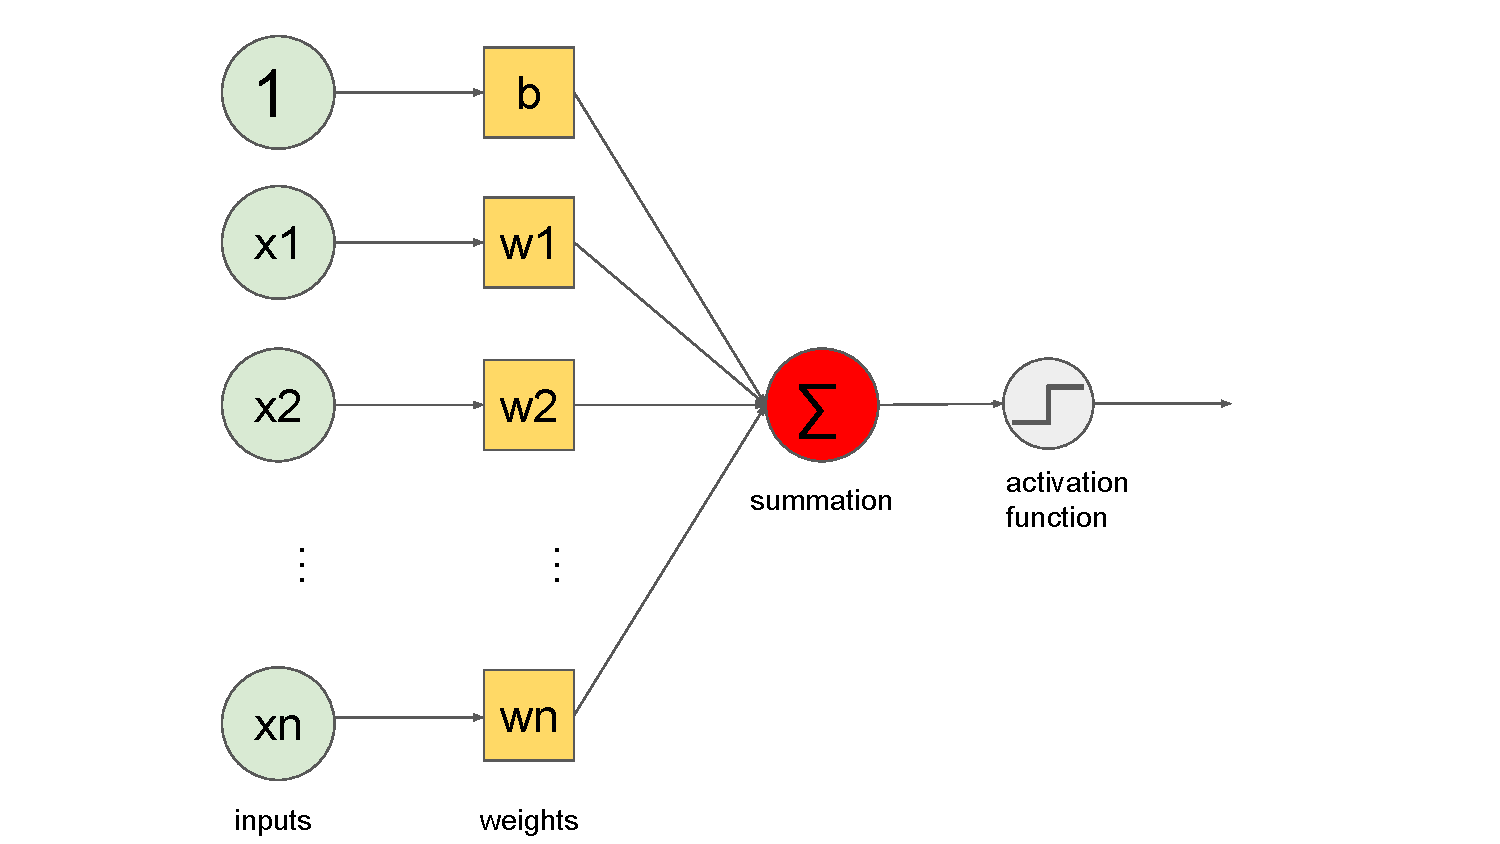
\includegraphics[width=\textwidth]{content/resources/new_images/related_works/perceptron.pdf}
    \caption{A single perceptron}
    \label{fig:perceptron}
\end{figure}

We first recap the early neural network, perceptron, which was introduced by Frank Rosenblatt in the 1950s \cite{rosenblatt1958perceptron} and 1960s \cite{rosenblatt1961principles}. 
The perceptron is an algorithm or a function for learning a binary classifier.
The function takes a $d$-dimensional vector $\mathbf{x}$ as input along with a weight vector $\mathbf{w}$ and calculates a single output value. 
\begin{align} \label{eqn: perceptron}
    a = f(\mathbf{x}) = \sigma(\mathbf{w}^T\mathbf{x} + b)
\end{align}
where $\mathbf{w}^T\mathbf{x} = \sum_{i=0}^{d} \omega_{i}x_{i} $ denotes the inner product between the input and weight vector and $b$ is bias. The perceptron behaves as a nonlinear function $\sigma$ of a linear combination of the input where each element $x_{i}$ is multiplied with it's corresponding coefficient $\omega_{i}$. 
Figure \ref{fig:perceptron} illustrates the process of a single perceptron process.\\
At first, the perceptron function is designed to solve the \textit{binary classification} problem in which each datapoint $\mathbf{x}$ belongs to a single class (denoted as \textbf{1} or \textbf{0}) and the weight vector $\mathbf{w}$ represents a boundary hyperplane that splits the space into two classes seperately. 
Therefore, points that lie at the same side of the plane are grouped to the same class. 
And the $sign$ function is used as activation function $\sigma$ in \ref{eqn: perceptron} to return $1$ if the combination is positive and $0$ otherwise.
\begin{align} \label{eqn: sgn_perceptron}
    a = f(\mathbf{x}) = \left\{\begin{matrix}
1 & \text{\quad if \quad} \mathbf{w}^T\mathbf{x} + b\geq 0 \\ 
0 & \text{\quad if \quad} \mathbf{w}^T\mathbf{x} + b <  0 
\end{matrix}\right.
\end{align}

\subsection{Activation functions}

Different from perceptron, activation function here is continuous, which makes the network weights differentiable with respect to output signals. \\
\begin{figure}[h]
    \centering
    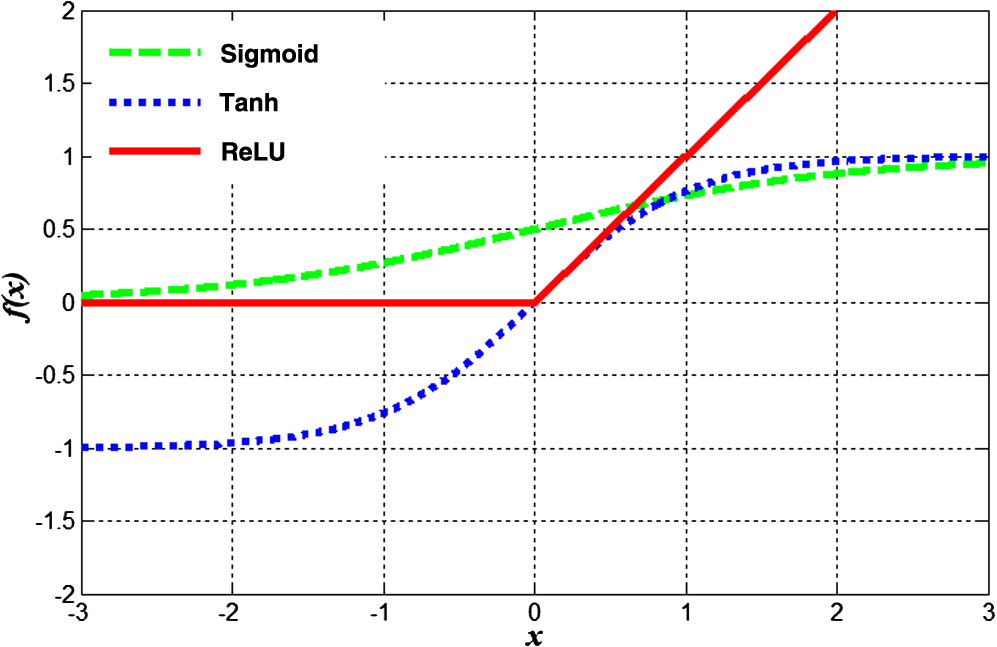
\includegraphics[width=0.7\textwidth]{resources/images/activation.png}
    \caption{Plot of Sigmoid, Tanh and ReLU activation functions.}
    \label{fig:activation}
\end{figure}
Here we list some of those activation functions commonly used in neural network modeling:
\begin{align} \label{eqn:sigmoid}
    \mathrm{sigmoid}(x) = \frac{1}{1 + \exp(-x)}
\end{align}
\begin{align} \label{eqn:tanh}
    \mathrm{tanh}(x) = \frac{\exp(2x - 1)}{\exp(2x + 1)} = 2 \times \mathrm{sigmoid}(2x) - 1
\end{align}
\begin{align} \label{eqn:relu}
    \mathrm{relu}(x) = \mathrm{max}(0, x)
\end{align}
The $sigmoid$ function (\ref{eqn:sigmoid}) scales real numbers to the range $[0, 1]$, where the large positive numbers change to $1$ and the large negative ones become $0$. Similar to $sigmoid$ but aims to produce zero-centered signals, $tanh$ function (\ref{eqn:tanh}) is a scaled version of $sigmoid$ with values range of $[-1, 1]$.\\
The drawback of both $sigmoid$ and $tanh$ is that when the numbers are large, the squashed values are saturated, hence their gradients is extremely small, which leads to the vanish problem when training deep neural networks. In such cases, Rectified Linear Unit ($ReLU$, \ref{eqn:relu}) is preferably used, which converts negative values to zero while keep the positive ones.
Figure \ref{fig:activation} illustrates the three functions in the same input range.



\subsection{Artificial Neural Networks}

The study of artificial neural networks (ANNs) has been inspired by the observation that biological learning systems are built of very complex webs of interconnected neurons in brains. The human brain contains a densely interconnected network of approximately trillion of neurons. ANN systems are motivated to capture this kind of highly parallel computation based on distributed representations. 

Generally, ANNs is a combination of a large number of interconnected processing neuron organized in a multi-layer architecture, where signal from a neuron can be passed to another from nearby layers (figure \ref{fig:neural_nets}). Each neuron is also formulated the same form as \ref{eqn: perceptron}. In general, neural network has an input layer, an output layer and a predefined number of hidden layers. Each hidden layer stands for a single transformation step in the process, which aims to extract hidden patterns of the input stored in it's neurons.  In recent years, state-of-the-art neural networks have multiple hidden layers. The number of layers determines the depth of the network, in contrast to the width of the network, which is determined by the maximum number of neurons between the hidden layers. In many cases, increasing depth increases the complexity of
the model, creates more space to store information and therefore increase its learning capability. These information is continually passed to following layers to extract more essential features. Due to the fact that sequence of linear transformations always equals to a single linear one, neural network uses nonlinear activation function $\sigma$ to element-wise apply to each processed neuron. 

\begin{figure}[h]
    \centering
    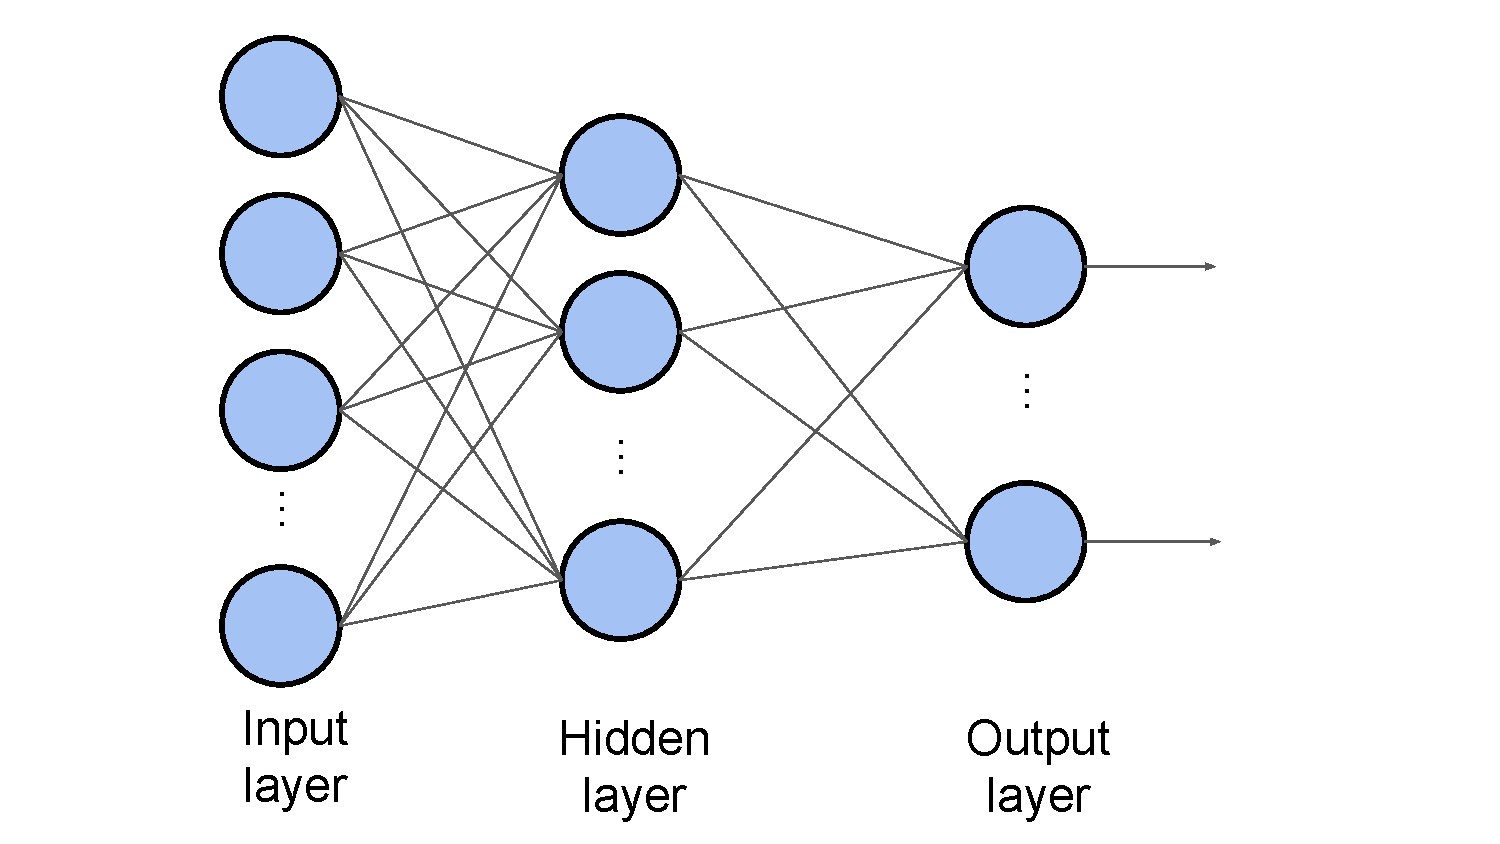
\includegraphics[width=0.7\textwidth]{content/resources/new_images/related_works/neural_nets.pdf}
    \caption{A simple three-layer neural network}
    \label{fig:neural_nets}
\end{figure}


Researchers have been actively conducting research on designing the architecture for ANNs to tackle machine learning and deep learning problem. Each new network design establishes on top of the older ones and each aims to solve a specific task independently. In order for the networks to deal with different tasks, such as classification, object detection, human action recognition, it cannot be without the usage of loss functions.

\subsection{Loss functions}

As stated in \ref{sec:ml}, supervised-learning neural networks must be trained with plenty of inputs-outputs data pairs. With every input, the network is expected to give a predictive outcome. While training, the network continuously adjusts its weights to minimize the discrepancy between its predicted outcome and the real outcome. The value of the discrepancy is often measured by using loss functions.

Loss functions are very diverse, each aims to solve different things and also is used for different tasks. For instance, in the regression task, the most used loss function is the least mean squared error. Suppose we have a model with parameters $\theta$, given a training sample $(x,y)$ where $x$ is the input and $y$ is the ground-truth, the loss for this single sample is calculated as follows

\begin{equation}
    \mathcal{L}(\theta,x,y) = \frac{1}{2} [y - h_{\theta}(x)]^2
\end{equation}

Similarly with classification task, the most frequently used one is cross-entropy loss. With the same notation as the example above, the loss function is as follows

\begin{equation}
    \mathcal{L}(\theta,x,y) = - (1-y_i) \text{log}(1-h_\theta(x_i)) - y_i\text{log}h_\theta(x_i)
\end{equation}

There are various factors involved in choosing a loss function for specific problem such as type of machine learning algorithm chosen, ease of calculating the derivatives and to some degree the percentage of outliers in the data set. 

So far, loss functions are used to determine the error between the output of our algorithms and the given target value. For the networks to perform better, it is essential to minimize the loss value. For only one training sample to be minimized, it is undoubtedly easy.
However, in practice, the loss value should be estimated for every possible training samples; this is nearly impossible. Therefore, the process of training can be formulated as an optimization problem: 

\begin{align}
    \mathcal{J}(\theta) &= E_{x,y} [L(\theta, x, y)] \approx \frac{1}{n} \sum^n_{i=1} L(\theta, x_i, y_i)
\end{align}

where $(x_i, y_i)$ is the $i^{th}$ oair and $n$ is the number of pairs in the dataset.
The target is to search for a set of parameters $\theta$ which minimize the expected loss function, or more realistically, calculate its approximation. An effective algorithm for this task is gradient descent, which is a fundamental tool of modern machine learning problems.

\subsection{Gradient descent}

Gradient descent (GD) is an iterative optimization algorithm used to find the local minimum of an objective function $J(\theta)$ by updating the parameters $\theta$ in the opposite direction of the gradient of that objective function. A gradient simply measures the change in all weights with regard to the change in error. In mathematical terms, a gradient is a partial derivative with respect to its inputs. 

How big the steps the GD takes into the direction of the local minimum are determined by the learning rate $\alpha$, which figures out how fast or slow we will move towards the optimal weights (as illustrated in Figure \ref{fig:gradient_descent}). Small value of $\alpha$ might lead to consistency but slow progress while larger one can result in faster progress but risk divergence. Thus, it must be carefully chosen. 

\begin{figure}[h]
    \centering
    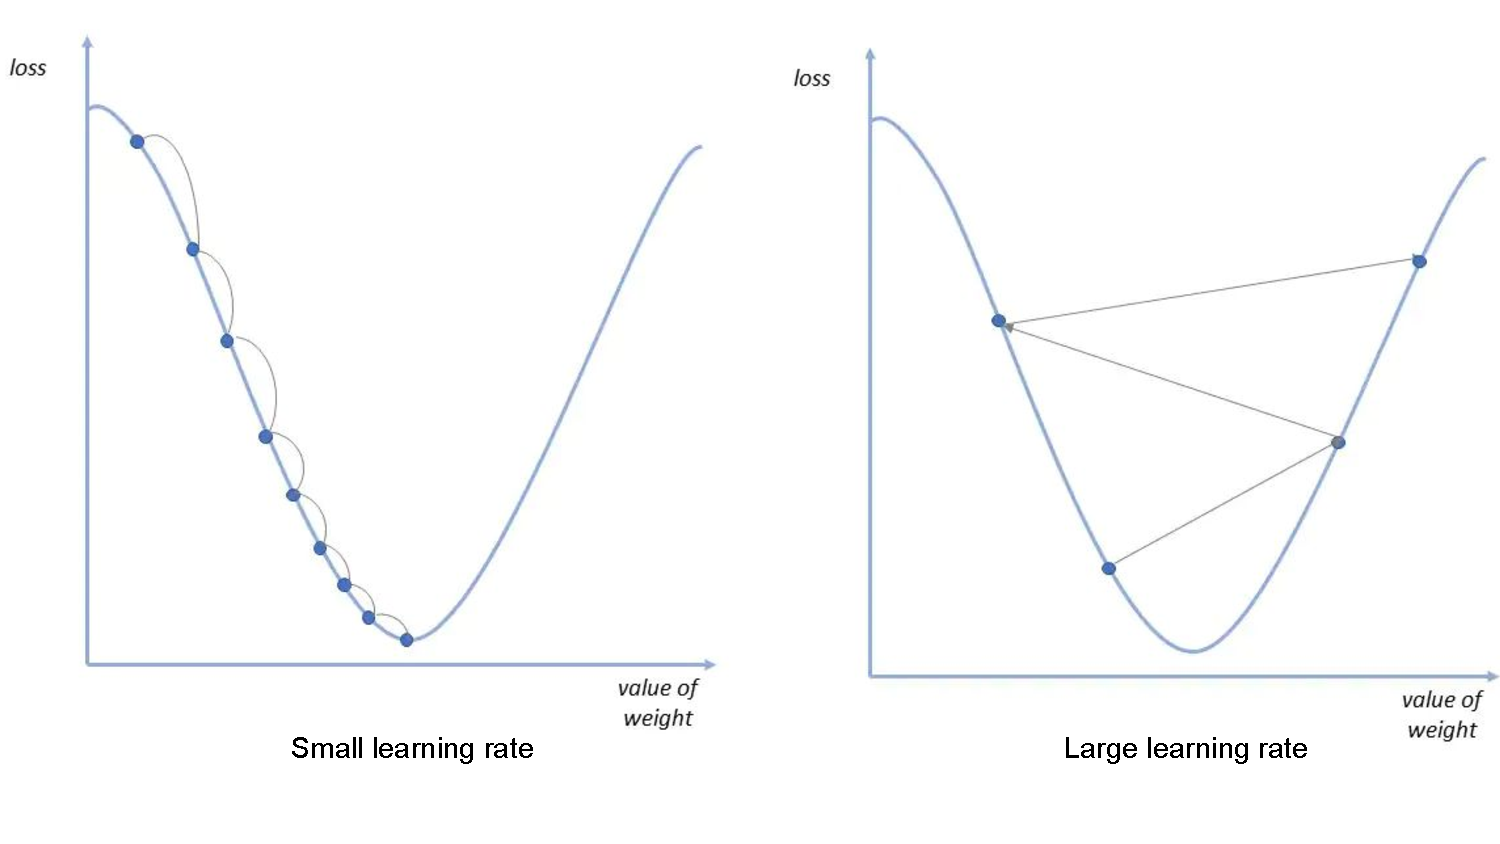
\includegraphics[width=0.9\textwidth]{content/resources/new_images/related_works/gradient_descent.pdf}
    \caption{Gradient descent}
    \label{fig:gradient_descent}
\end{figure}
 

Mathematically, the parameter $\theta_i$ in the set of parameters $\theta$ is updated as follows:

\begin{align}
    \theta_i := \theta_i - \alpha \frac{\partial J(\theta)}{\partial \theta_i}
\end{align}

While the original GD, also called vanilla GD, performs weights update after one pass through the whole dataset, which can be costly in practical scenario, there has been various variations that can alleviate this problem.
Stochastic gradient descent (SGD) \cite{bottou2010large} updates the parameters for each calculated training example one by one, which can help faster convergence than vanilla GD depending on the problem.  Additionally, the frequency of those updates can result in noisy gradients, which may cause the error rate to fluctuate instead of slowly decreasing. For the most strategic method, it must be the Mini-batch GD variant. It simply splits the training dataset into small batches and performs an update for each of those batches. From this variant, others with more parameters and mechanisms beside learning rate are introduced to improve the consistency and convergence speed of the algorithm, such as Adam \cite{kingma2014adam} or RMSProp.


\subsection{Feed-forward and Back-propagation}

\textbf{Feed-forward} describes the process of information flowing forward through the entire neural network. Given input data $x$, it is propagated through the intermediate layers to finally produce $\hat{y}$ at the output layer. Feed-forward is used both in the training and the testing phase to make predictions for any given input. In the training stage, the error is estimated between the network's output and ground truth; that essentially provides gradient information to update the network parameters. 

\textbf{Back-propagation} 
With the loss computed, back-propagation computes the gradient with respect to the weights of the network for a single input-output pair, and then flow the gradient information backward through the network . At each of the layers, new gradients are computed based on the following layers by the chain rule, then it is used to update the parameters in these layers using gradient descent. The process happens again until the gradients at the input layer are calculated and updated.

The process of feed-forward and back-propagation keep on repeating, and the weights keep updating continuously until the network becomes better fitted to the data that was fed into it, with reasonable evaluation result.

\section{Convolutional Neural Network}
\label{model:cnn}
Convolutional Neural Network (CNN or ConvNet) is a special case of fully-connected neural network discussed in previous session, which was specially designed to process grid-like topology data, such as images.
For example, with an image of size $[32, 32, 3]$, a single unit at first hidden layer in fully-connected neural network would have $32 \times 32 \times 3 = 3072$ weights corresponding to all the pixels. 
This amount increases exponentially with image size, the $[224, 224, 3]$ image would cost over $150000$ weights for each neuron. 
This make the network cost a lot of computation and easily overfit.
Furthermore, the traditional neural network views each image as a flatten vector, which may lead to lack of spatial information, given by groups of nearby pixels. Take inspiration from the biological visual system, each neuron in CNN only look at a restricted region (known as \textit{receptive field}) of the input image. \\
\begin{figure}[t!]
    \centering
    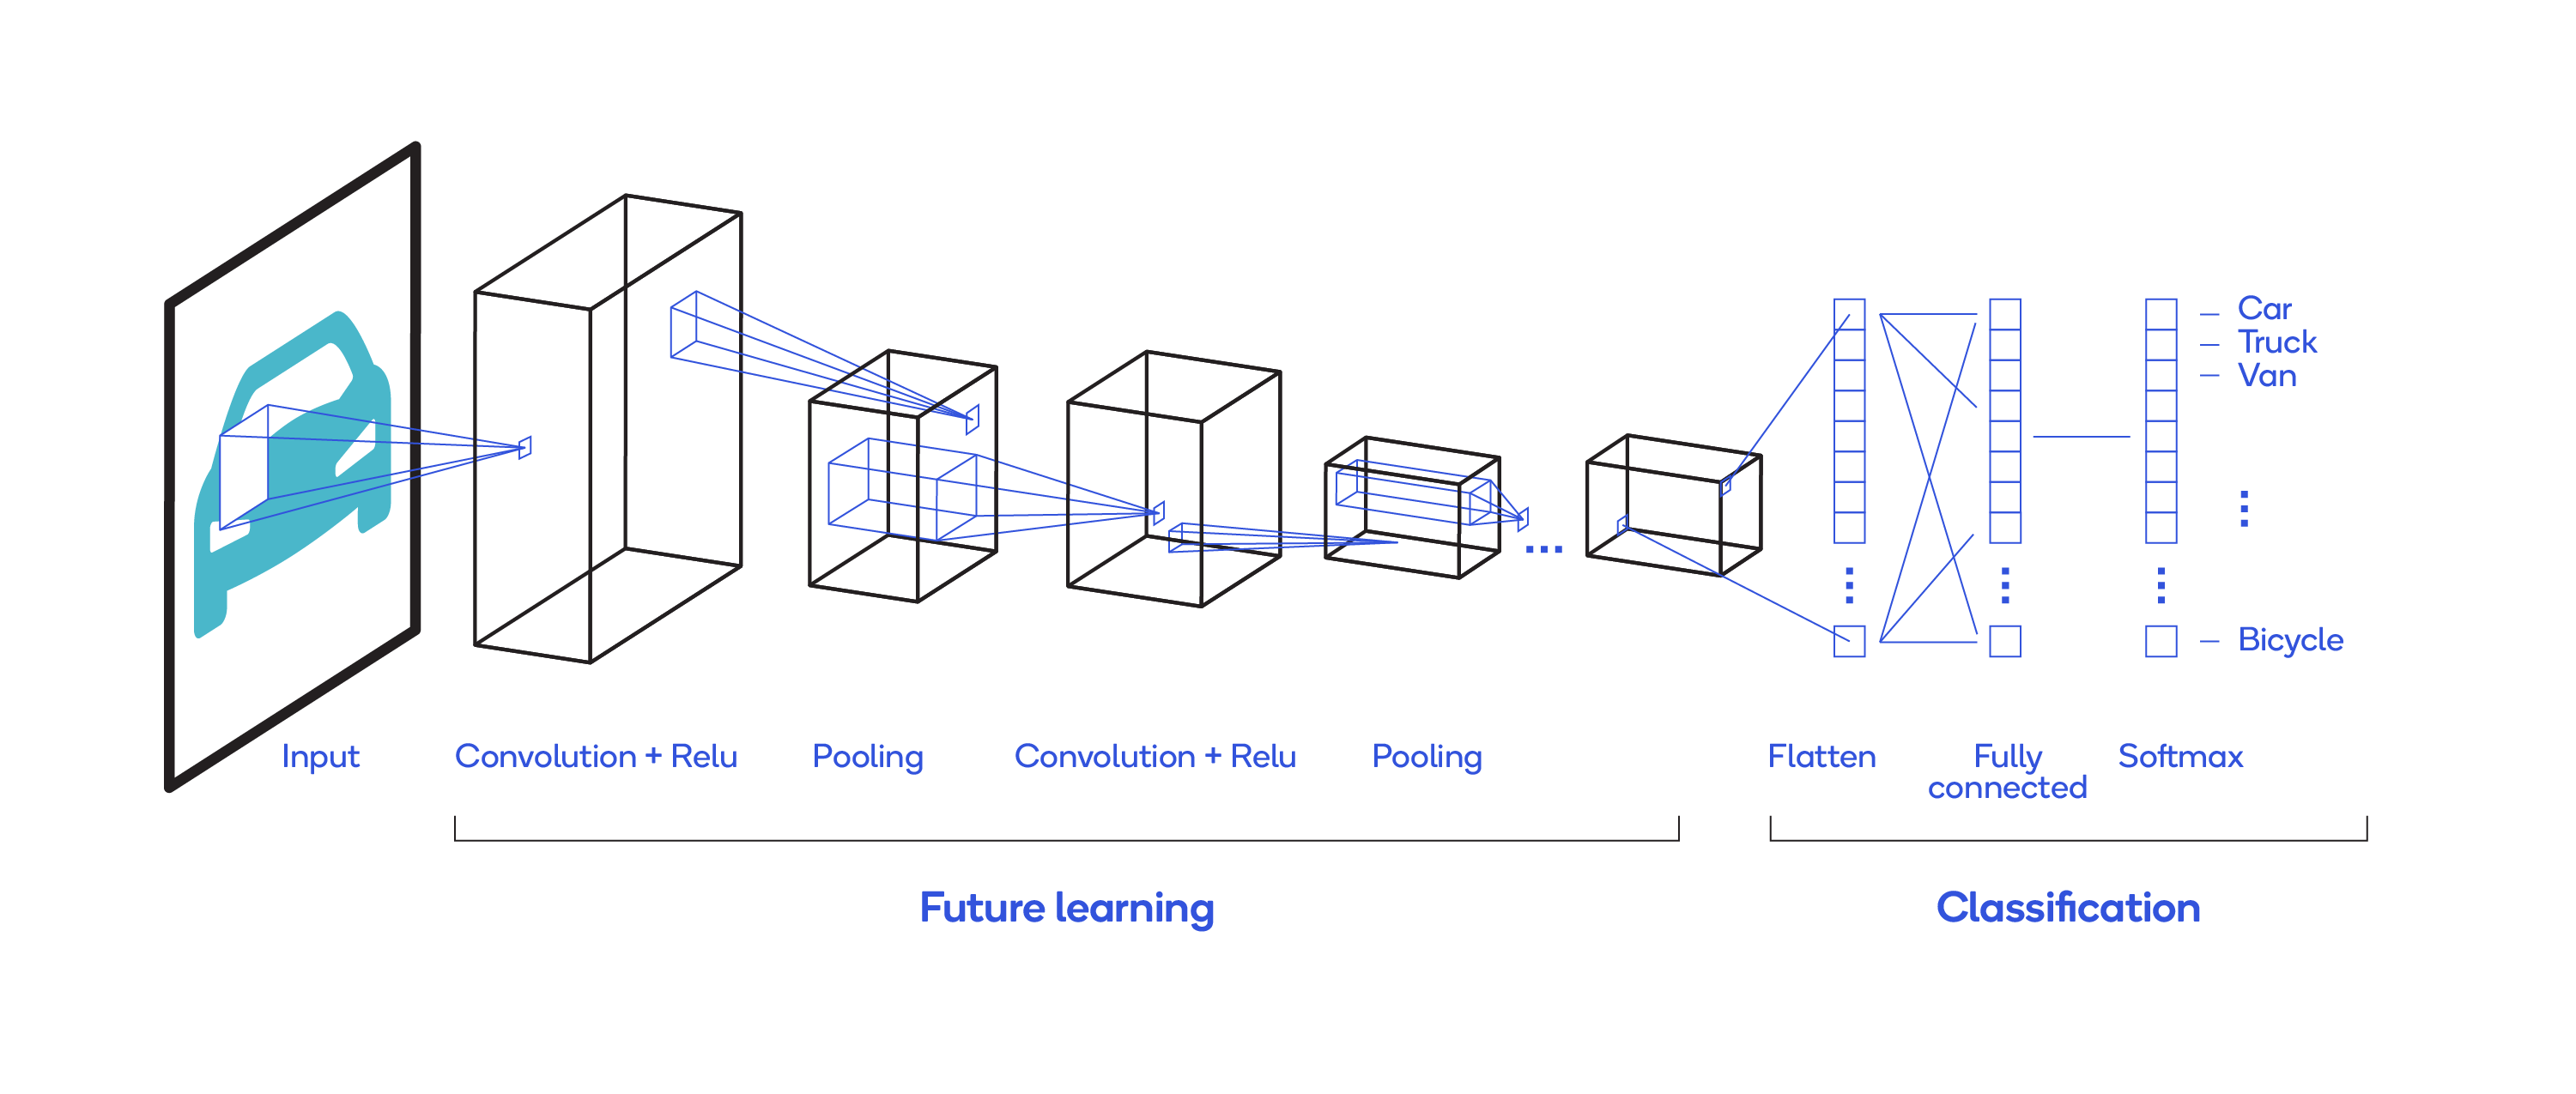
\includegraphics[width=\textwidth]{images/CNN.png}
    \caption{A neural network architecture for image classification task, constructed from convolutional layer, pooling layer and fully-connected layer.}
    \label{fig:cnn}
\end{figure}
Concretely, a simple ConvNet is constructed from a sequence of individual layers (illustrated in figure \ref{fig:cnn}): \\
\textbf{Convolutional Layer}. \quad The most important component in a CNN architecture. Receive an input volume from previous layer, the layer apply a convolution function using an adaptive \textit{kernel} (or \textit{filter}) to compute outcome neurons for current layer. The operation works as sliding the \textit{kernel} across the entire input then compute dot product between the covered input values and the filter entries. An activation function is also applied on each neuron value, as mentioned in \ref{model:mlp}. By this function, we output a 2D feature map with the shape usually smaller than the input volume. Intuitively, the convolution works as a pattern identifier, aims to extract visual feature given in images such as object edges or other special shapes, etc. \\
Some important hyper-parameters used to define a convolutional layer:
\begin{itemize}
    \item Kernel size: $[K \times K \times C_{in}]$, predefined shape of filter matrix used in convolution process. $C_{in}$ is the input channel of input tensor from previous layer.
    \item Number of kernel: $N_{k}$, the amount of kernels we apply at the current layer. Each kernel correspondents to a specific convolution layer, used to produce a 2D feature map. Finally, we stack these maps to achieve the output volume.
    \item Stride: $S$, the number of pixels that the kernel splits on the tensor.
    \item Padding: $P$, the number of rows/columns used to pad the input around the border. This step helps to reduce the information loss as the border pixels are not used as frequently as the inner ones.    
\end{itemize}
\textbf{Pooling Layer}. \quad The layer used to reduce the spatial size of the output feature map produced by successive convolutional layer. This technique helps to reduce computation cost and amount of parameters, and hence, help to control overfitting. \\
\textbf{Fully-Connected Layer}. \quad The layer performs exactly as a Neural Network mentioned in section \ref{model:mlp}. Receive the final representation from previous step, fully-connected layer provides a stack of dense connection to get the final prediction for a specific task. For example in image classification problem, the layer produce an output vector $\mathbf{o} \in \mathbb{R}^{c}$ ($c$ is the number of target classes), then apply a softmax function to give prediction confidence. \\
% Figure ... shows an example of a typical CNN architecture.\\
In general, ConvNet can be seen as a two-stage process, feature learning and prediction. The feature learning stage built from stack of convolution-pooling blocks, aims to produce the final representation of the input image while the prediction stage utilizes this embedded information for a specific tasks.
Therefore, the ConvNet is also commonly used for feature extraction and can be efficiently applied in various tasks such as Image/Video Retrieval, Instance Re-identification or Image Generation, etc. 

% \subsection{Modern convolutional networks}
% In this section, we 
% [TODO]
\section{Transformer}
\label{sec:transformer}
“Attention is All you Need” (Vaswani, et al., 2017) \cite{vaswani2017attention}, is impactful work in both natural language processing or computer vision field. It presented a lot of improvements and the proposed “transformer” model is entirely built on the self-attention mechanisms without using sequence-aligned recurrent architecture (which will describe in section \ref{subsec:attention}). The Transformer model has an encoder-decoder architecture, as commonly used in many natural machine translation models. Later decoder-only Transformer was shown to achieve great performance in language modeling tasks, like in GPT and BERT. Nowadays, transformer also use in computer vision because of the context-understanding ability of it and become one of the state-of-the-art.

\subsection{Sequence to sequence (Seq2Seq)}
The seq2seq model was introduced by Sutskever \cite{sutskever2014sequence}, et al in the language modeling field. It tackle the transformation of an source sequence to a target one, firsly apply in neural machine translation (figure \ref{fig:seq2seq}). The seq2seq model normally has an encoder-decoder architecture, composed of:

\begin{itemize}
    \item \textbf{Encoder}: to compress the information of input sequence and represent it as an context vector. This representation is expected to be summery the whole source sequence.
    \item \textbf{Decoder}: is initialized with the context vector to emit the transformed output. Seq2seq only used the last embedding state of the encoder network as the decoder initial input.
\end{itemize}
\begin{figure}
    \centering
    \includegraphics{}
    \caption{The sequence to sequence overview}
    \label{fig:seq2seq}
\end{figure}
This architecture is the foundation of many sequential models nowadays, but still exist few limitations such as use a fixed-length context vector. And one of the the most improvements handle this problem is attention mechanism.

\subsection{Attention and Self-Attention mechanism}
\label{subsec:attention}
\textbf{The attention mechanism} uses to memorize long source sentences in neural machine translation. Define the attention mechanism in a scientific way. Say, we have source sequence \mathbf{x} have length $n$ and target sequence \mathbf{y} have length $m$
\begin{equation}
\mathbf{x} &= [x_1, x_2, \dots, x_n] \text{;}
\mathbf{y} &= [y_1, y_2, \dots, y_m]
\end{equation}

The key idea is it create weighted shortcuts between the context vector and the entire source input. The alignment between the source and target is learned by a context vector. The context vector is a sum of hidden states $\boldsymbol{h}_i$ of the encoder sequence and weighted by alignment scores $\alpha_{t,i}$, in there $\alpha_{t_i}$ is calculate from the hidden states $\boldsymbol{s}_i$ from the decoder. 

\begin{equation}
\label{eq:align_score}
\mathbf{c}_t &= \sum_{i=1}^n \alpha_{t,i} \boldsymbol{h}_i & \small{\text{; Where $c_t$ is the context vector for output }y_t}
\end{equation}

The alignment score $\alpha_{t,i}$ is assign by a model to the pair of input at position and output at position based on how well they match. The set of pairs are weights how much of each source hidden state should be considered for each output. The score function is therefore in the following form below at timestamp $t$:
\begin{equation}
    e_{ij}=a(s_i,h_j), \qquad \alpha_{i,j}=\frac{\exp(e_{ij})}{\sum_k\exp(e_{ik})}
\end{equation}

\textbf{Self-attention} is an attention mechanism variant, in that it relating different positions of a single sequence in order to compute a representation of the same sequence. The self-attention mechanism use to learn the correlation between the current token and the previous part of the sequence. 

\subsection{Multi-head Self-Attention}
In the paper attention is all you need, transformer component have re-define the attention by using retrieval concept. The encoded representation of the input as a set of key-value pairs $\mathbf{K}, \mathbf{V}$.
In the decoder, the previous output is compressed into a query $\mathbf{Q}$ and the next output is produced by mapping this query and the set of keys and values.  

\begin{equation}
    \text{Attention}(\mathbf{Q}, \mathbf{K}, \mathbf{V}) = \text{softmax}(\frac{\mathbf{Q}\mathbf{K}^\top}{\sqrt{n}})\mathbf{V}
\end{equation}
Where $n$ is the dimension of the source hidden state. And we have a scalar score $a_{ij}$ follow
\begin{equation}
    a_{ij} = \text{softmax}(\frac{\mathbf{q}_i {\mathbf{k}_j}^\top}{\sqrt{n}})
= \frac{\exp(\mathbf{q}_i {\mathbf{k}_j}^\top)}{ \sqrt{n} \sum_{r \in S_i} \exp(\mathbf{q}_i {\mathbf{k}_r}^\top) }
\end{equation}
The reason behind this because the attention operation can be thought of as a retrieval process as well. As mention in eq \ref{eq:align_score}, if we remove the constraint that the weight $\alpha_{t}$ is a one-hot vector, the operation could be thought as a retrieval process according to the $\alpha_{t}$ as a probability vector. This way efficiency computes the vector $\alpha_{t}$ as a matrix multiply to measure the similarity by project $s$ and $h$ to a common space instead of we have to go through the network $n \times m$ times to acquire all the attention scores $a_{ij}$.
\begin{equation}
    \label{eq:scale_dot_product}
    \text{score}(\boldsymbol{s}_t, \boldsymbol{h}_i) = \frac{\boldsymbol{s}_t^\top\boldsymbol{h}_i}{\sqrt{n}}
    \caption{Scaled dot-product formula}
\end{equation}
\textbf{The multi-head self-attention module} is a key component in transformer. In summary, the idea of multi-head attention is to split the feature dimension of the input into many parts and attention over these sub-dimensions. Then computes the scaled dot-product attention (eq \ref{eq:scale_dot_product}) over each subspace in parallel. Each independent attention outputs are simply concatenated and linearly transformed into expected dimensions.
\begin{figure}[h]
    \centering
    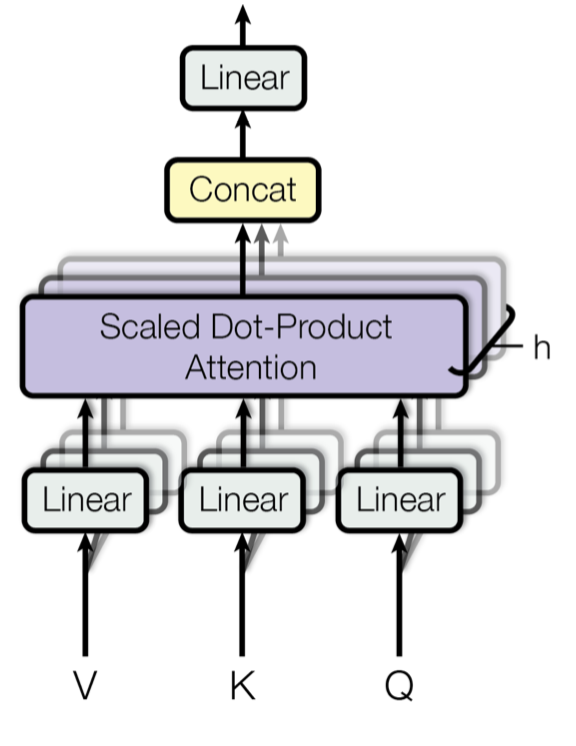
\includegraphics[height=2in]{content/resources/new_images/background/multi-head-attention.png}
    \caption{Multi-head scaled dot-product attention mechanism \cite{vaswani2017attention}}
    \label{fig:multiheadatt}
\end{figure}
\subsection{Transformer architecture}

\begin{figure}[h]
    \centering
    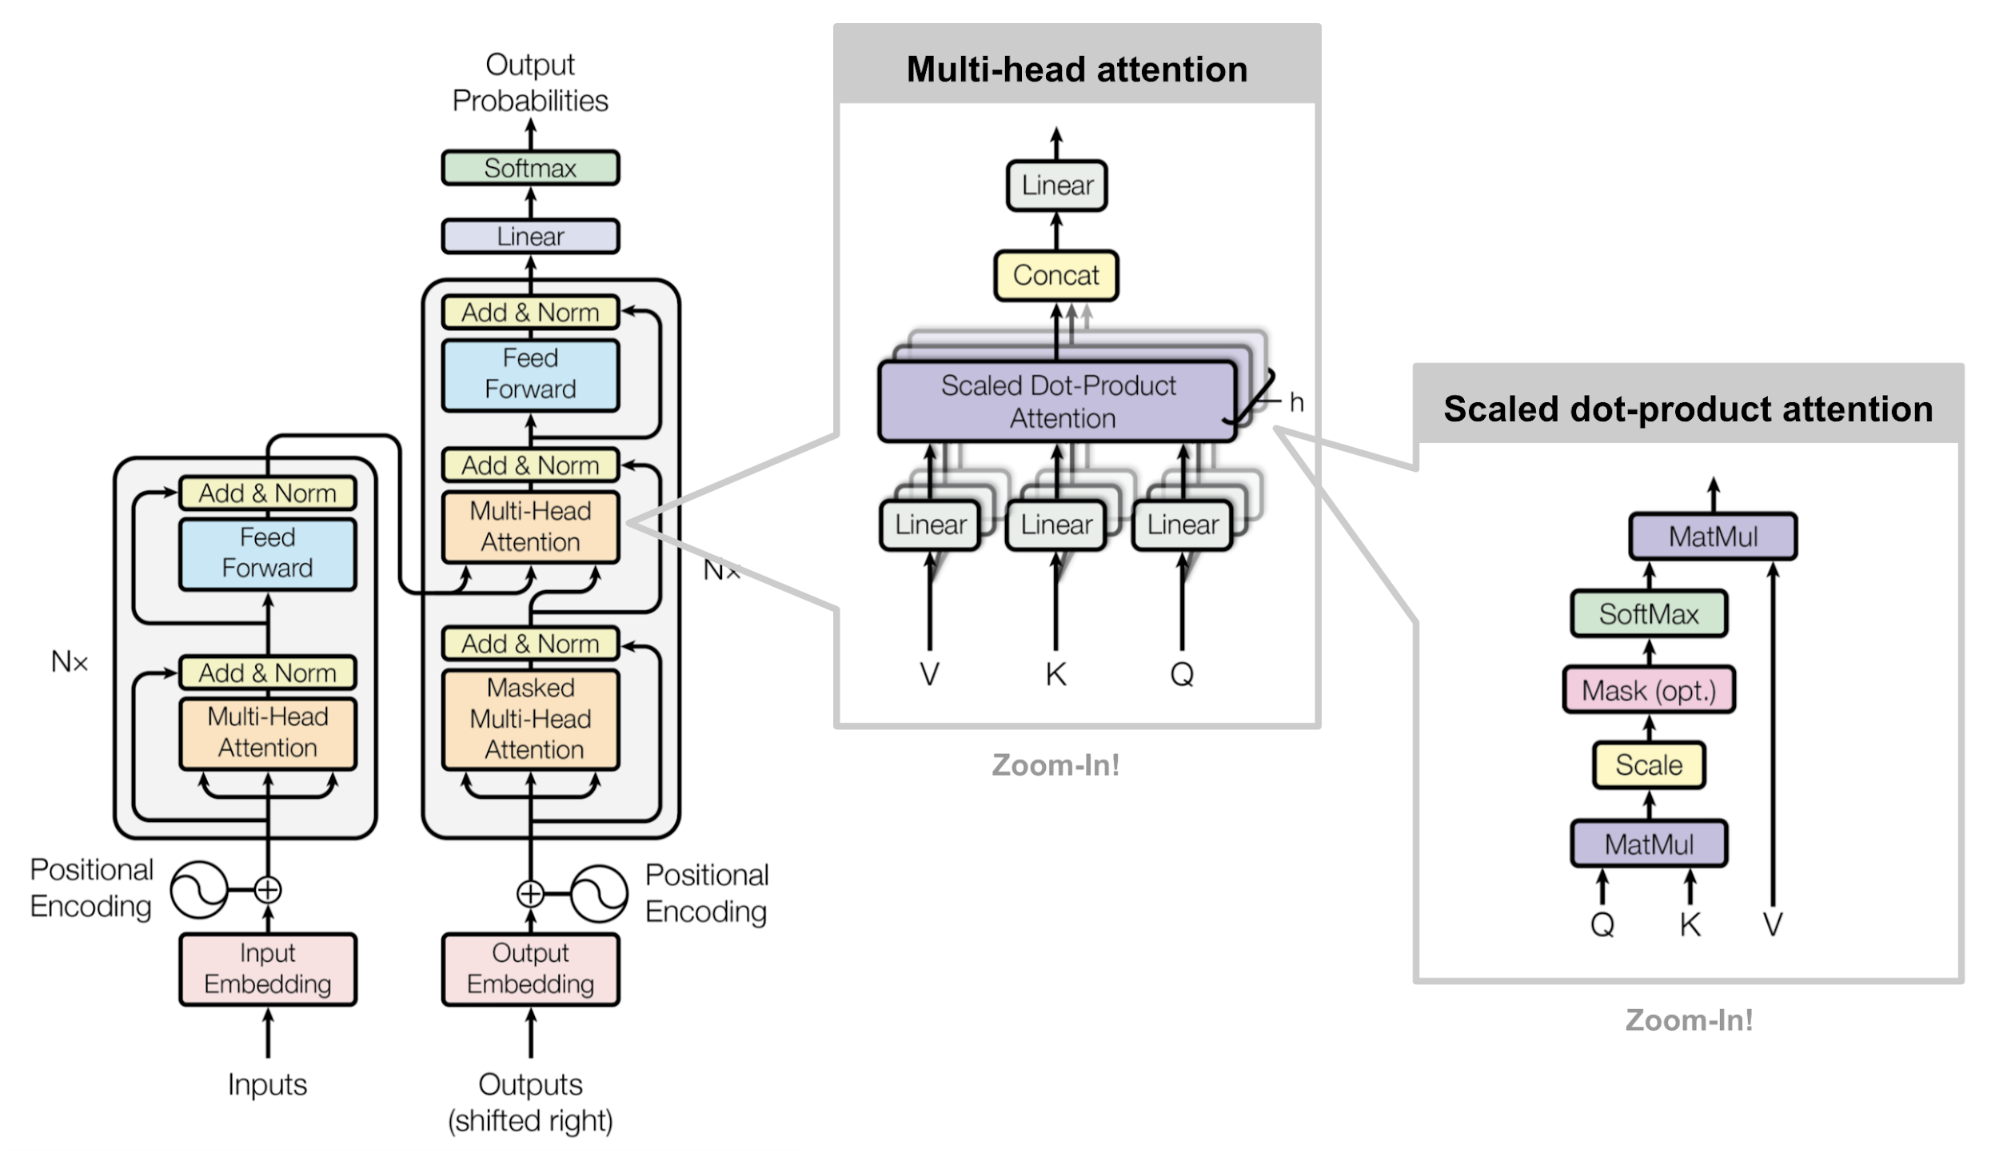
\includegraphics[width=\textwidth]{content/resources/new_images/background/transformer.png}
    \caption{The full transformer architecture \cite{vaswani2017attention}}
    \label{fig:transformer_arch}
\end{figure}


Transformer model has an encoder-decoder architecture. The encoder generates a representation from a large context. It constructed by two main submodules, a \textit{multi-head self-attention} layer and a \textit{projection network}. 

In the transformer decoder is retrieve information from the encoded representation. The architecture is quite similar to the encoder. Figure \ref{fig:transformer_arch} shown the whole propose architecture



